\documentclass[../main.tex]{subfiles}
\usepackage[utf8]{inputenc}
\usepackage[T1]{fontenc}
\usepackage{graphicx}
\usepackage{longtable}
\usepackage{wrapfig}
\usepackage{rotating}
\usepackage[normalem]{ulem}
\usepackage{amsmath}
\usepackage{amssymb}
\usepackage{capt-of}
\usepackage{hyperref}
\usepackage{float}
\graphicspath{{../}}
\author{Cezary Wieczorkowski}
\date{\today}
\title{Koncepcja}
\hypersetup{
 pdfauthor={Cezary Wieczorkowski},
 pdftitle={Koncepcja},
 pdfkeywords={},
 pdfsubject={},
 pdflang={Polish}}
\begin{document}


\section{Koncepcja nowego stanowiska}

\subsection{Założenia projektowe}

    Po przeanalizowaniu poprzedniego zestawu laboratoryjnego wypracowano następujące założenia dla projektu nowego zestawu:
    \begin{itemize}
    \item Zestaw musi zachować bloki funkcjonalne oraz zasadę działania poprzedniego zestawu.
    \item Zestaw ma zachować tryby pracy: cykl, mikrocykl oraz program.
    \item Zestaw musi emulować komponenty rzeczywistego układu szyny danych.
    \item Zestaw musi umożliwiać łatwą naprawę błędów w jego funkcjonowaniu oraz rozbudowę o nowe funkcjonalności.
    \item Zestaw musi zachować przejrzysty sposób wizualizacji stanu poszczególnych komponentów.
    \item Zestaw musi posiadać uniwersalny interfejs użytkownika pozwalający na łatwą obsługę zestawu oraz późniejsze jego modyfikacje.
    \end{itemize}

\subsection{Projekt sprzętowy}

    \subsubsection{Wybór mikrokontrolera}

    Ze względu na wybrane podejście symulacji programowej działania układu szyny danych, mikrokontroler jest centralnym elementem budowanego układu.
    W celu zapewnienia możliwości dalszej rozbudowy oraz wprowadzania poprawek do układu musi być to nowoczesna i łatwo dostępna platforma. 
    Istniejąca wersja zestawu jest oparta o mikrokontroler Atmega 8 oraz Atmega 32. Są to urządzenia pracujące z częstotliwością 16 MHz oraz 
    posiadające odpowiednio 1 Kb oraz 2 Kb pamięci RAM \cite{at:atmega8} \cite{at:atmega32}. Większość mikrokontrolerów dostępnych obecnie na 
    rynku oferuje znacząco większe możliwości. 
    \par
    Jako mikrokontroler do budowy zestawu wybrano układ RP2040 firmy Rassbery Pi \cite{rp:rp2040} obecny na płytce rozwojowej Rassbery Pi Pico. 
    Jest to układ oparty o architekturę ARM Cortex M0+, posiada 264 Kb pamięci RAM oraz pracuje z częstotliwością 133 MHz. Układ posiada duży zapas
    zasobów sprzętowych co pozwoli na szerokie możliwości rozbudowy zestawu w przyszłości. Dodatkowo dostępność układu na płytce rozwojowej uprości
    proces budowy sprzętowej części zestawu gdyż płytka ta zawiera wszystkie elementy niezbędne do pracy mikrokontrolera.

    \subsubsection{Elementy interfejsu użytkownika}

    Interfejs użytkownika zestawu powinien umożliwiać łatwą obsługę zestawu oraz umożliwiać łatwe wprowadzenie zmian w jego strukturze. Takie wymagania
    najlepiej spełni interfejs oparty o wyświetlacz wyświetlający menu z opcjami do wyboru oraz interfejs do nawigacji pomiędzy nimi. 
    Jako wyświetlacz zdecydowano się zastosować wyświetlacz znakowy LCD 20x4. Jest to wyświetlacz oparty o popularny układ sterujący HD44780 \cite{lcd_hd44780}.
    Dzięki prostocie obsługi oraz długiej obecności na rynku tego typu wyświetlacze są wspierane przez bardzo szeroką gamę oprogramowania.
    \par
    W celu nawigacji po menu zdecydowano się zastosować enkoder kwadraturowy. Jest to element generujący impulsy na podstawie ruchu obrotowego.
    Pozwala on na stwierdzenie kierunku oraz prędkości obrotu. Tego typu urządzenia stosowane są w układach sterowania pracą silników lub jako elementy
    wejściowe interfejsu użytkownika. Enkodery stosowane jako element nawigacyjny często posiadają wbudowany przycisk \cite{encoder} dzięki czemu obracając
    enkoderem można wybierać opcje menu a naciskając go można potwierdzać wybór.
    \par
    Dodatkowo w celu zapewnienia wizualizacji stanu elementów podczas pracy zestawu zdecydowano się ja w oryginale zastosować diody LED do 
    wizualizacji stanu adresów oraz słowa pamięci RAM, stanu rejestru $R_{WY}$ oraz wybranego rejestru ($R_A$, $R_B$, $R_C$).
    \par
    Jako elementy do wprowadzania danych binarnych zdecydowano się zachować przełączniki jak w oryginalnym zestawie. Dla uproszczenia obsługi zestawu
    dane do pamięci RAM oraz rejestru $R_P$ będą wprowadzane za pomocą jednego zestawu ośmiu przełączników natomiast dane użytkownika
    na szynę będą wprowadzana za pomocą osobnych czterech przełączników.

    \subsubsection{Dodatkowe peryferia}

    Sumując liczbę końcówek GPIO mikrokontrolera potrzebną do obsługi wybranych peryferiów otrzymujemy 43. 
    Mikrokontroler RP2040 posiada 30 końcówek GPIO \cite{rp:rp2040} co oznacza, że nie jest możliwe bezpośrednie podłączenie wszystkich peryferiów.
    W celu obsługi wszystkich peryferiów konieczne jest zastosowanie dodatkowych układów scalonych rozszerzających ilość dostępnych końcówek GPIO.
    \par
    Jednym z prostszych tego typu układów jest rejestr przesuwny. Jest to układ który posiada wejście zegarowe oraz wejście danych
    danych. Po każdym zboczu zegara dane z wejścia danych są przesuwane do kolejnej komórki rejestru. Niektóre rejestry przesuwne 
    posiadają wyjście danych z ostatniej komórki rejestru. Dzięki temu można połączyć kilka rejestrów kaskadowo. Jednym z takich układów jest
    74HC595 \cite{ti:74hc595}. Jest to 8 bitowy rejestr przesuwny z wyjściem równoległym. Rejestry te zastosowano do sterowania diodami LED. Użyto trzech
    układów ze względu na konieczność wysterowania 22 diod.
    \par
    W celu redukcji ilości końcówek GPIO potrzebnych do obsługi wyświetlacza LCD zdecydowano się zastosować ekspander I/O PCF8574 \cite{ti:pcf8574}.
    Jest to układ który pozwala na sterowanie 8 bitowym portem wejścia/wyjścia za pomocą interfejsu I2C. Dzięki temu obsługa wyświetlacza 
    zajmuje tylko dwie końcówki GPIO potrzebne do obsługi interfejsu I2C. 

    \subsubsection{Schemat blokowy sprzętowej części zestawu}

    Na rysunku \ref{fig:hardware_diagram} przedstawiono schemat blokowy sprzętowej części zestawu.
    
    \begin{figure}[H]
        \centering
        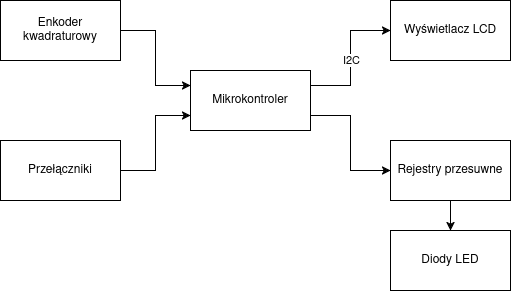
\includegraphics[width=\linewidth]{hardware_diagram.png}
        \caption{Schemat blokowy sprzętowej części zestawu}
        \label{fig:hardware_diagram}
    \end{figure}
    
\subsection{Architektura oprogramowania}

    \subsubsection{Struktura programu}

    Wybrany mikrokontroler RP2040 posiada dostarczane przez producenta SDK dla języka C/C++. W skład zestawu wchodzi szereg
    bibliotek pozwalających na obsługę peryferiów mikrokontrolera. Są to biblioteki niskopoziomowe o niewielkim stopniu abstrakcji.
    Znaczącym ograniczeniem SDK jest niewielka ilość bibliotek do obsługi urządzeń dołączanych do mikrokontrolera.
    W związku z tym do napisania oprogramowania zestawu zdecydowano się wykorzystać framework Arduino \cite{arduino_pico}. Jest to popularne środowisko 
    programistyczne wspierające wiele mikrokontrolerów oparte o język C++. Framework ten dostarcza wysokopoziomowe biblioteki do obsługi
    peryferiów mikrokontrolera. Ze względu na popularność Arduino framework dostępnych jest wiele bibliotek z nim kompatybilnych napisanych
    przez społeczność. 
    \par
    Oprogramowanie zestawu podzielono na kilka modułów odpowiadających za poszczególne funkcjonalności zestawu:

    \begin{figure}[H]
        \centering
        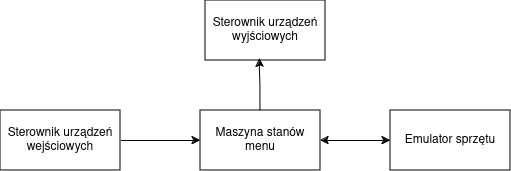
\includegraphics[width=\linewidth]{software_diagram.png}
        \caption{Schemat blokowy oprogramowania zestawu}
        \label{fig:software_diagram}
    \end{figure}

    \subsubsection{Emulacja elementów układu szyny danych}

    Wybrane podejście symulacji programowej układu szyny danych wymaga zaimplementowania emulacji poszczególnych elementów układu:

    \begin{itemize}
        \item Pamięci RAM
        \item Jednostki ALU wraz z komponentami pomocniczymi
        \item Mechanizmy sterujące pracą układu
        \item Rejestru $R_{WY}$
        \item Rejestru $R_P$
        \item Rejestru $R_A$
        \item Rejestru $R_B$
        \item Rejestru $R_C$
        \item Rejestru $R_I$
    \end{itemize}

    Rejestry oraz pamięć RAM są strukturami przechowującymi dane. Ich implementacje programowo można rozwiązać stosując zmienne które
    podobnie jak rejestry przechowują dane. Pamięć RAM oraz $R_P$ przechowuj więcej niż jedną wartość dlatego ich reprezentacje w 
    programie muszą być tablicami zmiennych o odpowiedniej długości. Symulacja jednostki arytmetyczno-logicznej wymaga implementacji
    operacji przez nią wykonywanych \ref{tab:operacje_alu}. Operacje te można zaimplementować z użyciem operatorów logicznych oraz arytmetycznych
    obecnych w języku C++. Kolejną częścią jednostki ALU jest system dekodowania słowa sterującego wyborem operacji oraz sposób pobierania
    wartości słowa sterującego z kolejnych instrukcji programu. Implementacja tego elementu wymaga zaimplementowania funkcji dekodującej.
    Ostatnią częścią konieczną do zaimplementowania jest system sterujące pracą układu. Kontrola pracy w pojedynczym mikrocyklu polega
    na zdekodowaniu pojedynczej instrukcji oraz wykonania na jej podstawie odpowiedniej operacji. Sterowanie pracą układu w trybach program
    oraz cykl można oprzeć na maszynie stanów która na podstawie aktualnego stanu układu oraz dokonuje odpowiednich przejść pomiędzy stanami.

    \subsubsection{Obsługa peryferiów sprzętowych}

    Oprogramowanie układu musi obsługiwać następujące peryferia:

    \begin{itemize}
        \item Wyświetlacz LCD
        \item Enkoder kwadraturowy
        \item Przełączniki
        \item Układy 74HC595 - diod LED
    \end{itemize}
    Przełączniki są podłączone bezpośrednio do końcówek GPIO mikrokontrolera więc ich status można odczytać za pomocą funkcji
    dostarczonych przez framework Arduino. Diody LED są sterowane za pomocą układów 74HC595. Sterowanie tymi układami wymaga 
    generacji sygnału zegarowego oraz wystawiania kolejnych bitów danych na wejście danych układu zgodnie z taktem zegara.
    Zdecydowano się użyć biblioteki implementującej ten protokół w środowisku Arduino framework \cite{arduino_74hc595}.

    Obsługa wyświetlacza LCD odbywa się poprzez ekspander I/O PCF8574. Komunikacja z ekspanderem odbywa się za pomocą interfejsu I2C.
    Do obsługi wyświetlacza wykorzystano bibliotekę kompatybilną z frameworkiem Arduino - LiquidCrystal PCF8574 \cite{lcd_pcf8574}. 
    Enkoder kwadraturowy jest obsługiwany za pomocą biblioteki wybranej do implementacji systemu menu opisanej w dalszej części dokumentu.

    \subsubsection{Obsługa interfejsu użytkownika}
    Interfejs użytkownika powinien udostępniać użytkownikowi następujące funkcje:
    \begin{itemize}
        \item Wybór trybu pracy zestawu
        \item Zapis oraz odczyt RAM oraz $R_P$
        \item Wprowadzanie danych na szynę
        \item Wizualizacja stanu elementów układu
        \item Wybór aktualnie wyświetlanego rejestru
    \end{itemize}
    Wizualizacja stanów elementu układów jest realizowana za pomocą diod LED, pozostałe funkcjonalności należy zaimplementować w oparciu
    o wyświetlacz LCD oraz enkoder. Zdecydowano się  zastosować interfejs użytkownika w formie menu. Menu jest to element interfejsu 
    użytkownika składający się z szeregu opcji pomiędzy 
    którymi użytkownik może nawigować. Opcje te po wybraniu mogą prowadzić do kolejnych poziomów menu lub wykonywać konkretne akcje.
    W tym przypadku do menu będzie wyświetlane na wyświetlaczu LCD a nawigacja będzie odbywać się poprzez obrót oraz naciśnięcie enkodera.
    Na rysunku \ref{fig:menu_diagram} przedstawiono strukturę menu dla projektowanego zestawu.

    \begin{figure}[H]
        \centering
        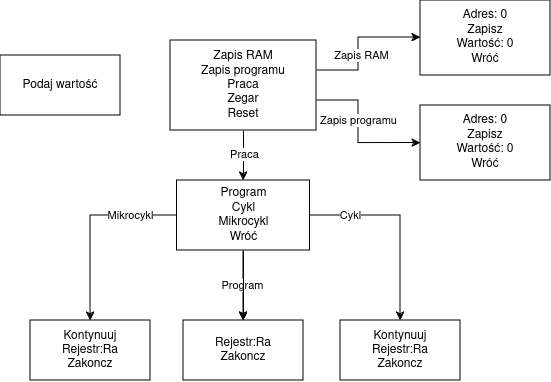
\includegraphics[width=\linewidth]{menu_diagram.png}
        \caption{Diagram menu interfejsu użytkownika}
        \label{fig:menu_diagram}
    \end{figure}

    Pierwszym menu widocznym dla użytkownika jest ogólny ekran nawigacyjny prowadzący do pozostałych opcji. Z jego poziomu można przejść
    do zapisu/odczytu pamięci RAM oraz $R_P$, wyboru trybu pracy zestawu oraz zresetować zestaw. Z poziomu ekrany wyboru trybu pracy można 
    rozpocząć pracę zestawu w jednym z trzech dostępnych trybów. Podczas pracy w dowolnym trybie użytkownik ma możliwość natychmiastowego 
    zakończenia pracy zestawu oraz wyboru aktualnie wyświetlanego rejestru. W trybach cykl oraz mikrocykl znajduje się dodatkowa opcjami
    "Kontynuuj" po wciśnięciu której zestaw wykonuje kolejny cykl/mikrocykl. Ostatni dostępny ekran jest wywoływany w przypadku
    gdy program działający na zestawie w danej instrukcji czyta dane z klawiatury "Dane". Program jest zatrzymywany a użytkownik jest proszony
    o wprowadzenie danych. Po zatwierdzeniu przez użytkownika zestaw kontynuuje pracę.

    Do programowej implementacji systemu menu zdecydowano się wykorzystać bibliotekę Arduino menu \cite{arduino_menu}. Jest to biblioteka
    pozwalająca na implementacje hierarchicznego systemu menu w prosty sposób. Posiada ona szereg wbudowanych prymitywów pozwalających
    na łatwą implementacje opcji menu pełniących funkcje takie jak: wywołanie przypisanej funkcji, zmiana wartości zmiennej lub przejście
    do kolejnego poziomu menu. Dużą zaletą tej biblioteki są wbudowane sterowniki dla wielu urządzeń wejścia oraz wyjścia. Biblioteka 
    bez natywnie wspiera obsługę enkodera kwadraturowego oraz wyświetlacza LCD za pomocą biblioteki LiquidCrystal PCF8574 \cite{lcd_pcf8574}.

\end{document}